\documentclass[a4,center,fleqn]{NAR}
\usepackage[pdftex,
colorlinks=true, %makes the links show up in color, rather than in a box
citecolor=black, %color of the in-text citation numbers
urlcolor=blue %color of the url links
]{hyperref}


\bibliographystyle{unsrt}

% Enter dates of publication
\copyrightyear{}
\pubdate{}
\pubyear{}
\jvolume{}
\jissue{}

%\articlesubtype{This is the article type (optional)}

\begin{document}

\title{PEACE: {\underline P}arallel {\underline E}nvironment for {\underline A}ssembly
  and {\underline C}lustering of Gene {\underline E}xpression}

\author{D.M. Rao\,$^{1}$, J.C. Moler\,$^{1}$, M. Ozden\,$^1$, Y. Zhang\,$^{1}$,
  C. Liang$^{1,2*}$\, and J.E. Karro\,$^{1,3}$\footnote{to whom
    correspondence should be addressed}}

\address{$^1$ Department of Computer Science and Software Engineering, \\
  $^2$ Department of Botany, \\
  $^3$ and Department of Microbiology, Miami University, Oxford, Ohio,
  USA}



\history{Received Feb. 12, 2010}

\maketitle

\begin{abstract}
  We present {\sc Peace}, a tool for the high-throughput clustering of
  transcript fragment sequences produced Next Generation or Sanger
  Sequencing technologies.  Installed and easily run through an easily
  downloaded GUI, {\sc Peace} can process large data sets, grouping the
  fragments by gene association, faster and with greater sensitivity
  than competing clustering tools such as {\sc WCD}, and with
  considerably greater sensitivity than the implicit clustering
  preformed by assembly tools such as {\sc Cap3}.  Through the GUI the
  user can collect cluster statistics and examine specific
  clusters for more comprehensive study.  And by using {\sc Peace} as
  a ``pre-assembly'' tool to allow the application of an assembly tool
  to the resultant individual clusters, the user gains both a significant
  increase sensitivity of the clustering method and a large decrease
  in overall runtime for the clustering and assembly together.
\end{abstract}


\section{Introduction}

Understanding an organism's transcriptome, the set of (spliced)
transcripts expressed by genes of the organism, is a vital step in
understanding the full functional and organization roll of the genome
in the life cycle of any organism.  Studying the transcriptome has led
to gene discovery, provided information of protein isoforms, and
generally helped shed light on the biological processes both
controlling and dictated by the genome \cite{Nagaraj07}.  But in order
to get access those transcripts, we must first deal with the
fragmented data produced by both Next Generation and traditional
Sanger sequencing technology.

Until recently, a primary method of gaining access to a transcriptome
sequence was through the use of Express Sequence Tags (ESTs), which
were primarily single-pass cDNA sequences derived from transcribed
mRNAs and traditionally sequenced by Sanger Sequencing technology.
More recently, Next-Generation Sequence (NGS) technologies have
replaced the Sanger Sequencing techniques, allowing for considerably
greater depth and coverage of the transcriptome.  For example, ESTs in
GenBank dbEST are increasingly the product of NGS technologies such as
454 pyrosequencing, which enables the sequencing of novel and rate
transcripts at a considerably higher rate of coverage than did Sanger
Sequencing \cite{Cheung2006,Emrich2007}.  But from a computational
perspective, this is a mixed blessing: while NGS provides immense
quantities of new information, it does provides immensely larger data sets
for analysis, requiring even more efficient algorithms than were
already needed.

Given a set of transcript fragments, produced by either sequencing
technology, sampled from multiple transcripts across the genome, a
necessary first step is that of clustering: separating the fragments
according to the transcript from which they were derived.  While
clustering is frequently preformed implicitly by assembly tools such
as {\sc Cap3} \cite{Huang99}, clustering the data as a
``pre-assembly'' step has a number of advantages.  Most significant
among these: preforming this step will allow the application of the
assembly tool to individual clusters -- saving significant amounts of
time due to the reduced input size \cite{Hazelhurst08a}.  But
clustering is a computationally challenging problem, especially when
done {\it ab initio} instead of relying on access to a sequenced
genome.  Even with the number of ESTs produced using Sanger
sequencing, the runtime and memory requirements to cluster based on
pair-wise sequence alignments make such an approach infeasible.  The
much larger data-set sizes produced by the next-generation sequencing
technologies exacerbates this problem.

Here we present {\sc Peace}, a tool for the {\it ab initio} clustering
of transcript fragments by gene, applicable to both short-read and traditional
Sanger Sequencing technologies.  Available through the
\href{http://www.peace-tools.org}{www.peace-tools.org} website, the PEACE GUI allows the user
to both easily install (locally or remotely) and run the computational
tool, as well as providing various tools for result analysis. {\sc
  Peace} can be run in single or multi-processor mode, and requires no
Internet connectivity past the initial download.  Using a {\it minimum
  spanning tree} (MST) based clustering strategy \cite{Jain99,Wan08}
and the $d^2$ sequence distance function \cite{Hide94}, {\sc Peace}
generates the MSTs using a tailored version of Prim's algorithm
\cite{Prim57}.  The result is an easy-to-use clustering tool that is considerably
more sensitive to sequencing errors than the competing {\sc wcd} tool
\cite{Hazelhurst08a} and others in the literature without any
sacrifice of performance (e.g. \cite{Burke99}, \cite{Slater00},
\cite{Huang99}, \cite{Parkinson02}, \cite{Kalyanaraman03},
\cite{Malde03}, \cite{Ptitsyn05}, \cite{Picardi09}).

\enlargethispage{-65.1pt}

\section{PEACE: Instillation and Use}

The {\sc Peace} GUI, available from the {\sc Peace} website
(\href{http://www.peace-tools.org}{www.peace-tools.org}), handles the
details of both instillation and job management and provides tools for
the initial analysis of the results.  By downloading and executing the
{\tt peace.jar} GUI Java program on a Linux, Windows or OS-X machine
running Java 1.6+, the user is presented with the {\sc Peace}
management tool.  Through this the user can install the computational
tool and preform a clustering of a data file, view an initial analysis
of the clusters and produce files containing subsets of the clusters
for assembly by a tool such as {\sc Cap3} \cite{Huang99}.  A typical
(first) use of the tool would generally require the the following
steps.

\noindent {\bf Tool Instillation:} Installing the GUI requires only
that the Java file be downloaded from the website.  To install the {\sc
  Peace} tool onto a local or remote machine, the user will select
from within the GUI the {\tt Server > Add New Server} tab from the GUI
main menu (Figure~1(a)), which then starts the install
wizard that will prompt for the appropriate information.
Figure~1(b) illustrates the request for server information;
in this example, the user has chosen to install the {\sc Peace}
computational tool on a remote machine and is providing the necessary
connection information.  Server information is persistent between GUI
sessions, giving the user access to {\sc Peace} on the target machine
as needed.

\noindent {\bf Job Processing:} After importing the target file into
the GUI ({\tt File > New Data Set}), the user can start a new job with
the {\tt Job > Job to Complete Clusters} tab and follow the wizard
menus.  Figure~1(c) illustrates the process of specifying
the number of processors available (if running on a machine supporting
the OpenMPI protocol -- which will be determined during job
instillation).  Once executed, the GUI will manage the job thread,
alert the user when the job is completed (or when the user next
runs the GUI after completion) and 
copy the final results back to the local machine if necessary.

\noindent {\bf Result Analysis:} Once the resulting clusters have been
computed and (if necessary) copied back, the user has several options
for analysis:
\begin{itemize}
\item {\bf Export:} The user can export the contents of one or more
  clusters into a fasta file, obtaining a subset of the original file
  containing the sequences corresponding to the selected clusters
  ready for processing by an assembly tool (e.g. {\sc Cap3} \cite{Huang99}).
\item {\bf View Clustering}: The user may view a list of all clusters,
  expanding selected clusters to a list of all fragments (illustrated in
  Figure~1(d)).  
\item {\bf Classified Summary Graph:} The user may view a distribution
  of cluster sizes in a linear or $\log$ scale.  Further, the user may
  set up a {\it classifier}, associating certain patterns with
  specific colors.  These patterns will be matched against the
  fragment header information from the original fasta file, allowing
  the overlay of a colored cluster size distribution does clusters
  containing matching elements in a specified colors.  For example, if
  the sequence names contain unique string patterns denoting different
  cDNA libraries, the classifier can help the user to determine the
  differential expression profiles of different libraries for a given
  cluster by color coding the strains.  The method of setting up a
  these classifiers, and the resulting histogram, is illustrated in
  Figure~1(e).
\end{itemize}

Extensive documentation for the tool has been posted on the {\sc
  Peace} website, as well as links to several videos demonstrating
{\sc Peace} use and capabilities.


\section{Methods}

The clustering performed by {\sc Peace} is based on the use of minimum
spanning trees (MSTs), known to be an effective approach for narrow
band single linkage clustering \cite{Jain99,Wan08}. We use the $d^2$
distance measure \cite{Hide94} to represent edge weights.  Prim's
algorithm \cite{Prim57} then allows us to efficiently calculate an
MST from which we can infer a high-quality clustering solution.

The $d^2$ distance measure used to assign edge weights is an
alignment-free measurement of sequence distance that can be calculated
significantly faster than a Smith-Waterman alignment
\cite{Hide94,Foret09}.  $d^2$ works by comparing the frequency of
words (strings of a fixed length) appearing in a limited region of
each string.  Fragments overlapping by a sufficient length will share
neighborhoods of enough similarity to ensure a small distance even in
the presence of a moderate number of base errors.  Our method of
calculating $d^2$, the {\it two-pass $d^2$ heuristic}, is a refinement
of that used in the {\sc wcd} clustering tool \cite{Hazelhurst08a}.  We
augment the computation with a preliminary pass that narrows down the
two regions of maximum similarity, and then explore those local
regions in more detail.

We can model the fragment input as a weighted, undirected graph: the fragments
are represented as nodes, with $d^2$ sequence distances assigned to
the connecting edges as weights.  Conceptually, we want to remove each
edge exceeding a threshold score from the complete graph, and define
our partitions by the remaining connected components of the graph.  An
edge with a large weight connects fragments which are likely unrelated;
once such edges are removed, the components define a series of
overlaps.  Hence those fragments that can still be connected by some path
correspond to the same gene.  However, such an approach requires the
calculation of all edge weights.  Such a task is infeasible both in terms of
runtime and memory usage for the data set sizes we expect to process.

We approach the problem by generating a minimum spanning tree of the
described graph, then removing edges exceeding our threshold.  By
using Prim's algorithm we are able to calculate edge weights
on-the-fly (reducing memory requirements), and we can skip the
calculation of a majority of edge distances using the $u/v$ and $t/v$
filtering heuristics employed in {\sc wcd} \cite{Hazelhurst08a}.
These heuristics allow us to quickly dismiss many of the edges as too
large without the need to apply the full $d^2$ algorithm (see
Sections~A and B of the Supplementary Materials for more details). 

\section{Results}

We have tested {\sc Peace} on both simulated and real data,
comparing results against those produced by the {\sc wcd}
clustering tool \cite{Hazelhurst08a} and the {\sc Cap3} assembly
tool \cite{Huang99} (which calculates a cluster as an intermediate
step).  For our simulation tests we used the {\bf ESTSim} tool
\cite{Hazelhurst03} to generate simulated transcript fragments under varying models
of error (Supplementary Materials, Section~\href{ESTsim_sup}),
generating the fragments from the list of 100 zebra fish genes used in
the {\sc wcd} testing \cite{Hazelhurst08a}.  Tool parameters were
taken to match, as closely as possible, those used in the {\sc wcd}
study (see supplementary materials).  Our primary methods of quality
assessment were {\it sensitivity} (the fraction of fragment pairs from the
same gene that were correctly clustered together) and {\it Type 1
  error} (the fraction of genes that were divided between clusters)
\cite{Wang04,Hazelhurst08a}; other measurements are also discussed
in the supplementary materials.  In Figure~2(left) we see a
significant improvement of {\sc Peace} (blue) over {\sc wcd}
(green) and {\sc Cap3} (black) in its sensitivity to sequencing
errors, while in Figure~2(right) we see a comparable
improvement in Type 1 error.  In Figure~3 we look at
the number of singleton clusters (fragments not joined to any cluster),
which will not occur in our simulated sets; we again see significant
improvement in {\sc Peace}.  The sequential runtime of
{\sc Peace} is slightly improved over that of {\sc wcd} (see
Supplementary Materials, Figure~S4).

\begin{figure*}[b]
\centerline{
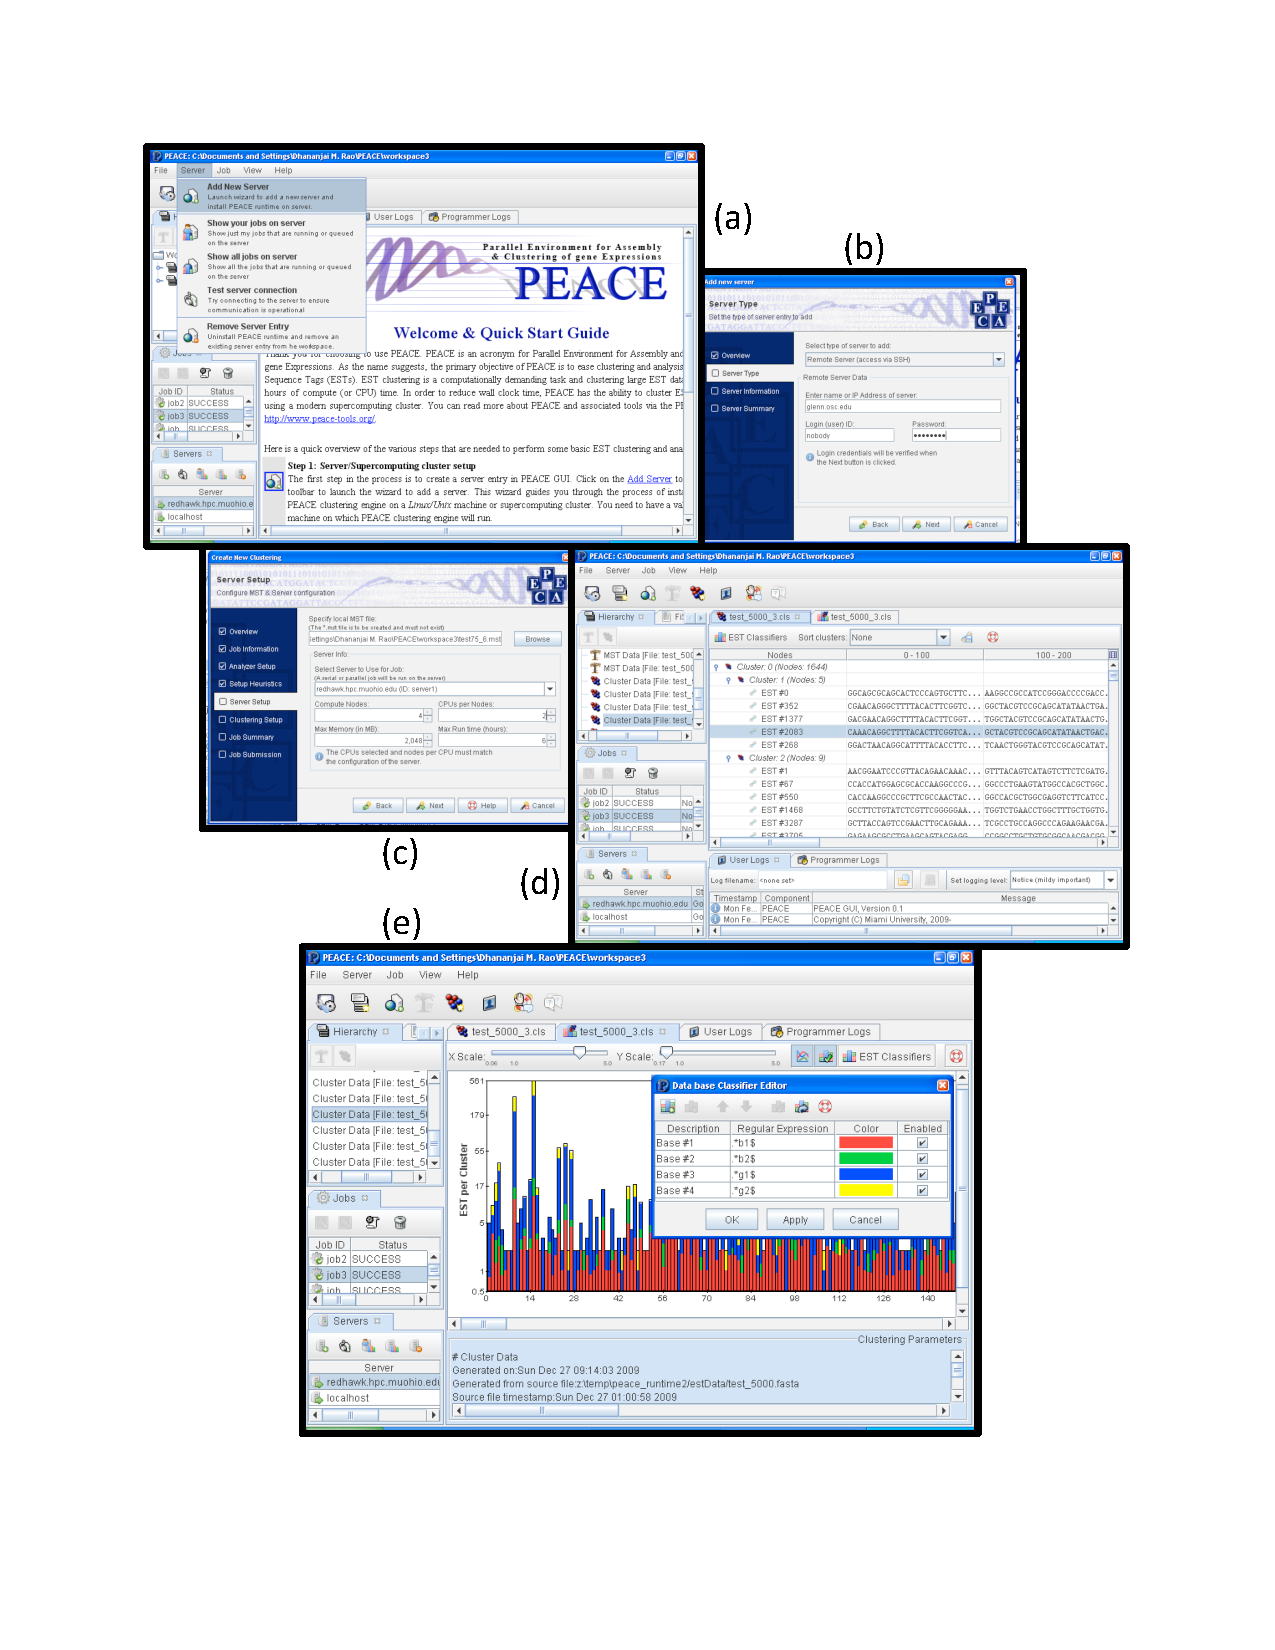
\includegraphics[trim=0cm 3cm 0cm 1cm, clip, scale=0.9]{screen.d/screen.pdf} 
}
\label{screen}
\caption{Screenshots of the PEACE GUI during execution, including (a)
GUI Welcome and server instillation menu; (b) setup wizard for
installing the computational tool on a remote server; (c) execution
wizard for starting a selected job to be executed in parallel mode;
(d) basic cluster output; and (e) histogram view of cluster results
and classifier editor for setting up differential expression profiles.}
\end{figure*}

\begin{figure*}[b]
\centerline{
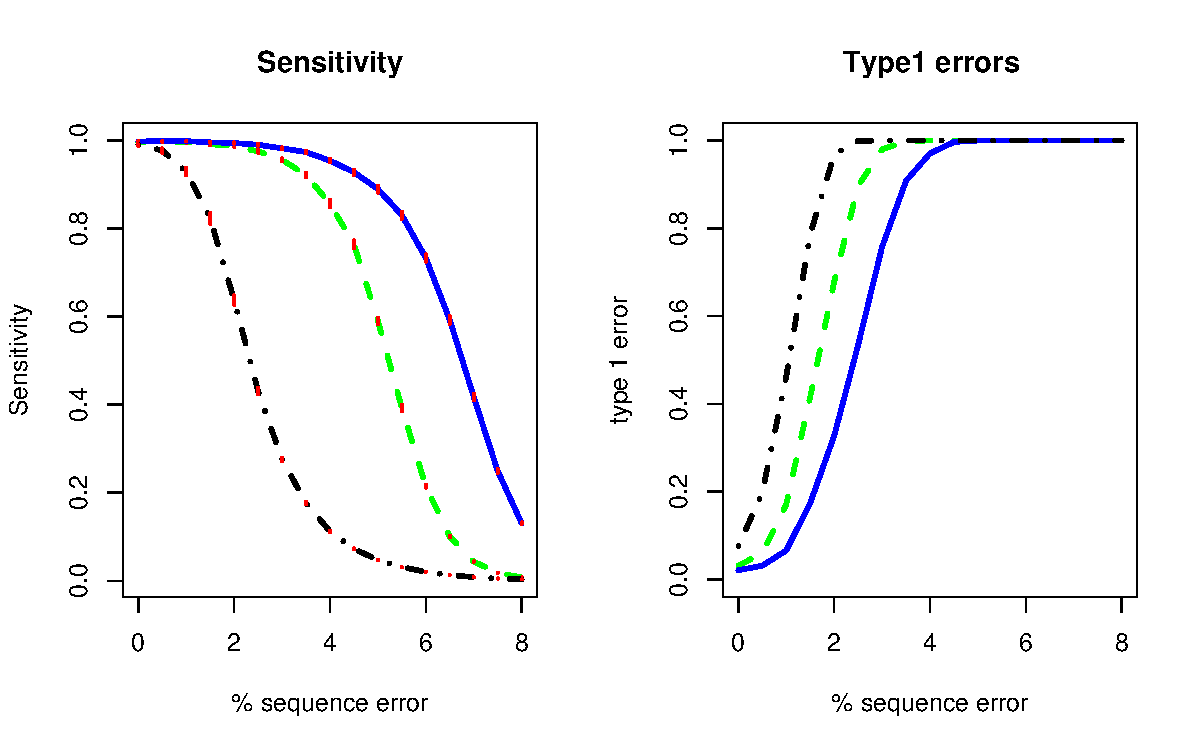
\includegraphics[scale=0.5]{pics.d/SeT1.pdf} 
}
\label{SeT1}
\caption{Comparisons of Sensitivity and Type 1 error, based on the
  average over 30 Simulated fragment sets derived from 100 zebra fish genes
  (see Supplementary Materials, Section~\href{sim_results}, for more
  details).   Blue/Solid = {\sc Peace}, Green/Dash =
  {\sc wcd}, Black/Dot-Dash = {\sc Cap3}; vertical tics = 95\% confidence
  intervals on estimates.  Intervals are not presented for Type 1
  error due to the extremely small variance.}
\end{figure*}

\begin{figure*}[b]
\centerline{
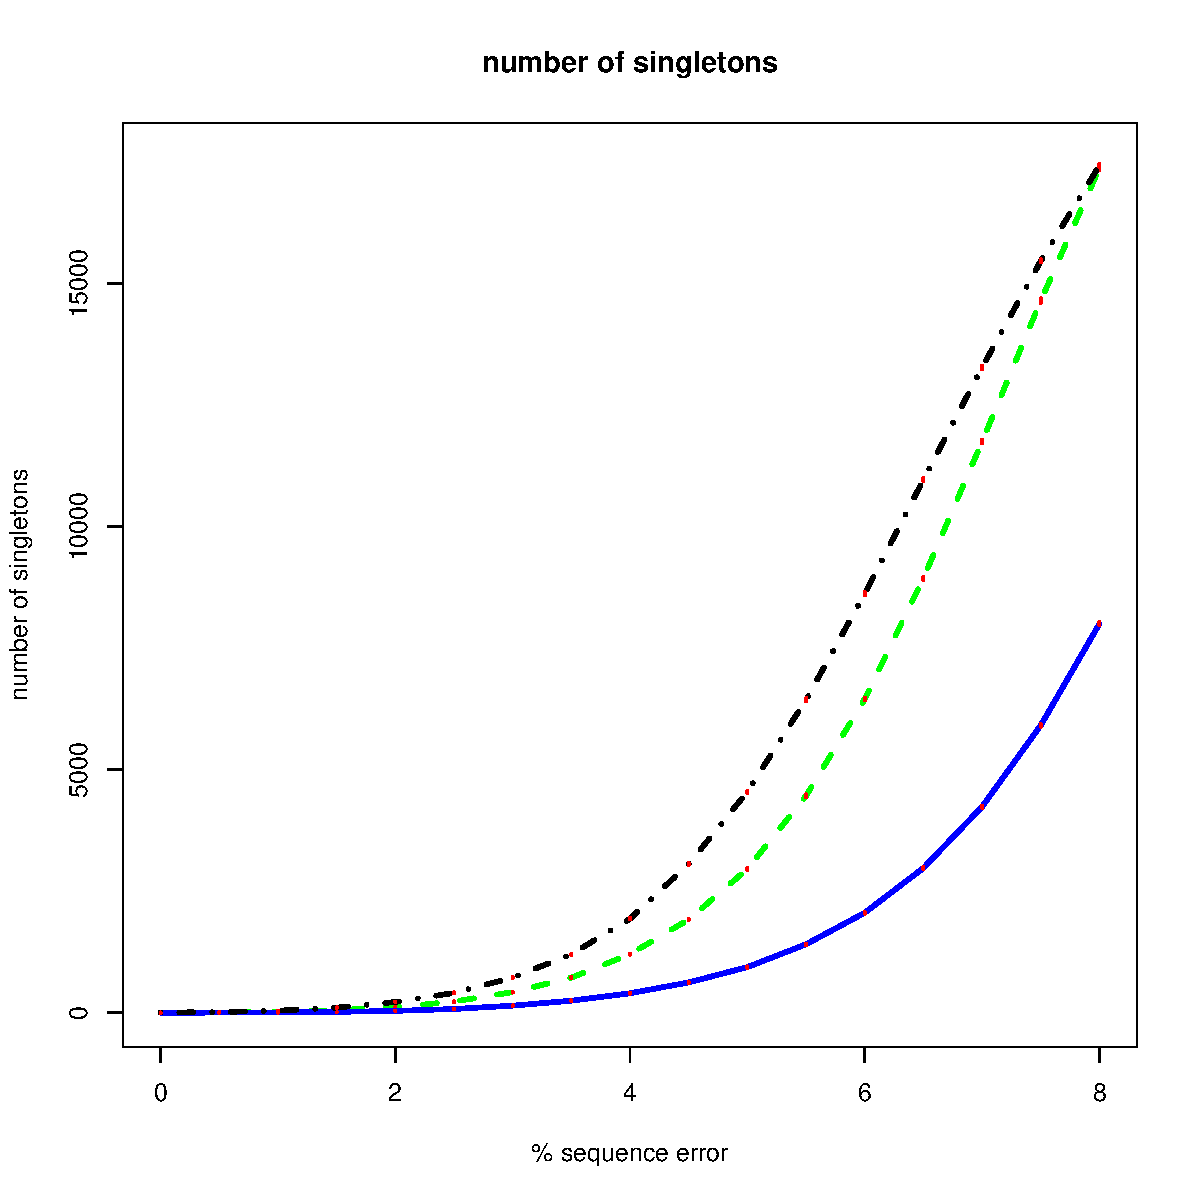
\includegraphics[scale=0.35]{pics.d/singletons.pdf}
}
\label{singletons}
\caption{Average number of fragments flagged as singletons by each tool
  when run on the simulated sequences; correct answer in all cases is
  zero.  Blue/Solid = {\sc Peace}, Green/Dash = {\sc wcd},
  Black/Dot-Dash = {\sc Cap3}.}
\end{figure*}

In applying the tools to real data, we started with a set of
approximately $190,000$ clean Sanger ESTs derived from the {\it
  Chlamydomonas reinhardtii} genome \cite{Liang2008}.  To compute
sensitivity we used the {\it gmap} tool \cite{Wu05} to map the
fragment set to the genome, taking this as our reference clustering.
We see slight improvements in {\sc Peace} over {\sc wcd} in both
sensitivity and Type 1 error (both significantly out preforming {\sc
  Cap3}).  Using the mouse fragment set used in Hazelhurst {\it et
  al.}  \cite{Hazelhurst08a} {\sc Peace} again shows slight
improvements in sensitivity and Type 1 error rates, with an 18\% speed
up for {\sc Peace} (see Supplementary Materials,
Section~\href{real_results}, for more details).

\section{Acknowledgements}

Dr. Karro was funded under a PhRMA Foundation Informatics Research
Starters Grant while conducting this research.  We would also like to
acknowledge Iddo Friedberg, David Woods, Jens Mueller and David
Scoville at Miami University for their help with this project.

\vspace{3mm}
%Bib TeX

\bibliography{peace.bib}



\end{document}


% LocalWords:  arallel nalysis lustering ngine Rao Moler Ozden Zhang Liang ESTs
% LocalWords:  Karro XXXXX transcriptome pre isoforms SNPs unsequenced runtime
% LocalWords:  chlamydomondomonas ESTate PaCE xsact CLU WCD Hazelhurst et al th
% LocalWords:  CHUN nalyzer Prim's MSTs subgraph MPI SourceCode ESTSim runtimes
% LocalWords:  ests Chlamydomonas Reihartdii gmap CDNA transcriptomes cDNA www
% LocalWords:  reinhartdii conifergdb DNAc bp wcd reinhardtii PhRMA Iddo fasta
% LocalWords:  Friedberg Scoville OpenMPI initio multi Screenshots nvironment
% LocalWords:  ssembly xpression GenBank dbEST pyrosequencing ESTsim sim
